\section{Magnetism and mean field theory}\label{sec:magMFT}

In this section we will build a picture of magnetism in the Hubbard model in increasing level of sophistication.
As our degenerate perturbation theory  calculation of section (\ref{sec:effectiveHeisenber}) showed, the on-site interaction favors the situation in which neighboring fermions have opposite spins through an Heisenberg type interaction.
A different approach leads to the Stoner criterion for ferromagnetism.
The argument is based on creating an imbalance between the numbers of spin-up and spin-down fermions, and analyzing the interplay between the resulting increase in kinetic energy, and decrease in potential energy.
Finally, we formulate a (static) mean field theory for the Hubbard model, and discuss how it relates to the non-interacting case.

\subsection{Stoner criterion for ferromagnetism}
\label{subsec:stoner}

Pauli's exclusion principle gives a prescription on how to fill fermionic energy levels so as to yield the lowest possible total energy.
Start from the lowest level, and start filling each level of higher energy consecutively with two electrons, one of each spin.
This procedure requires the number of spin-up and spin-down electrons to be the same.
Otherwise, there is an energy cost, since we are obliged to fill higher energy levels with the excess electrons.

An unequal number of spin-up and spin-down electrons also decreases the potential energy.
An extreme example is a completely polarized lattice.
In that case, the potential energy is zero.
Partial spin polarization makes double occupation unlikely, lowering the potential energy.

\begin{figure}[H]
	\centering
\hspace{12mm}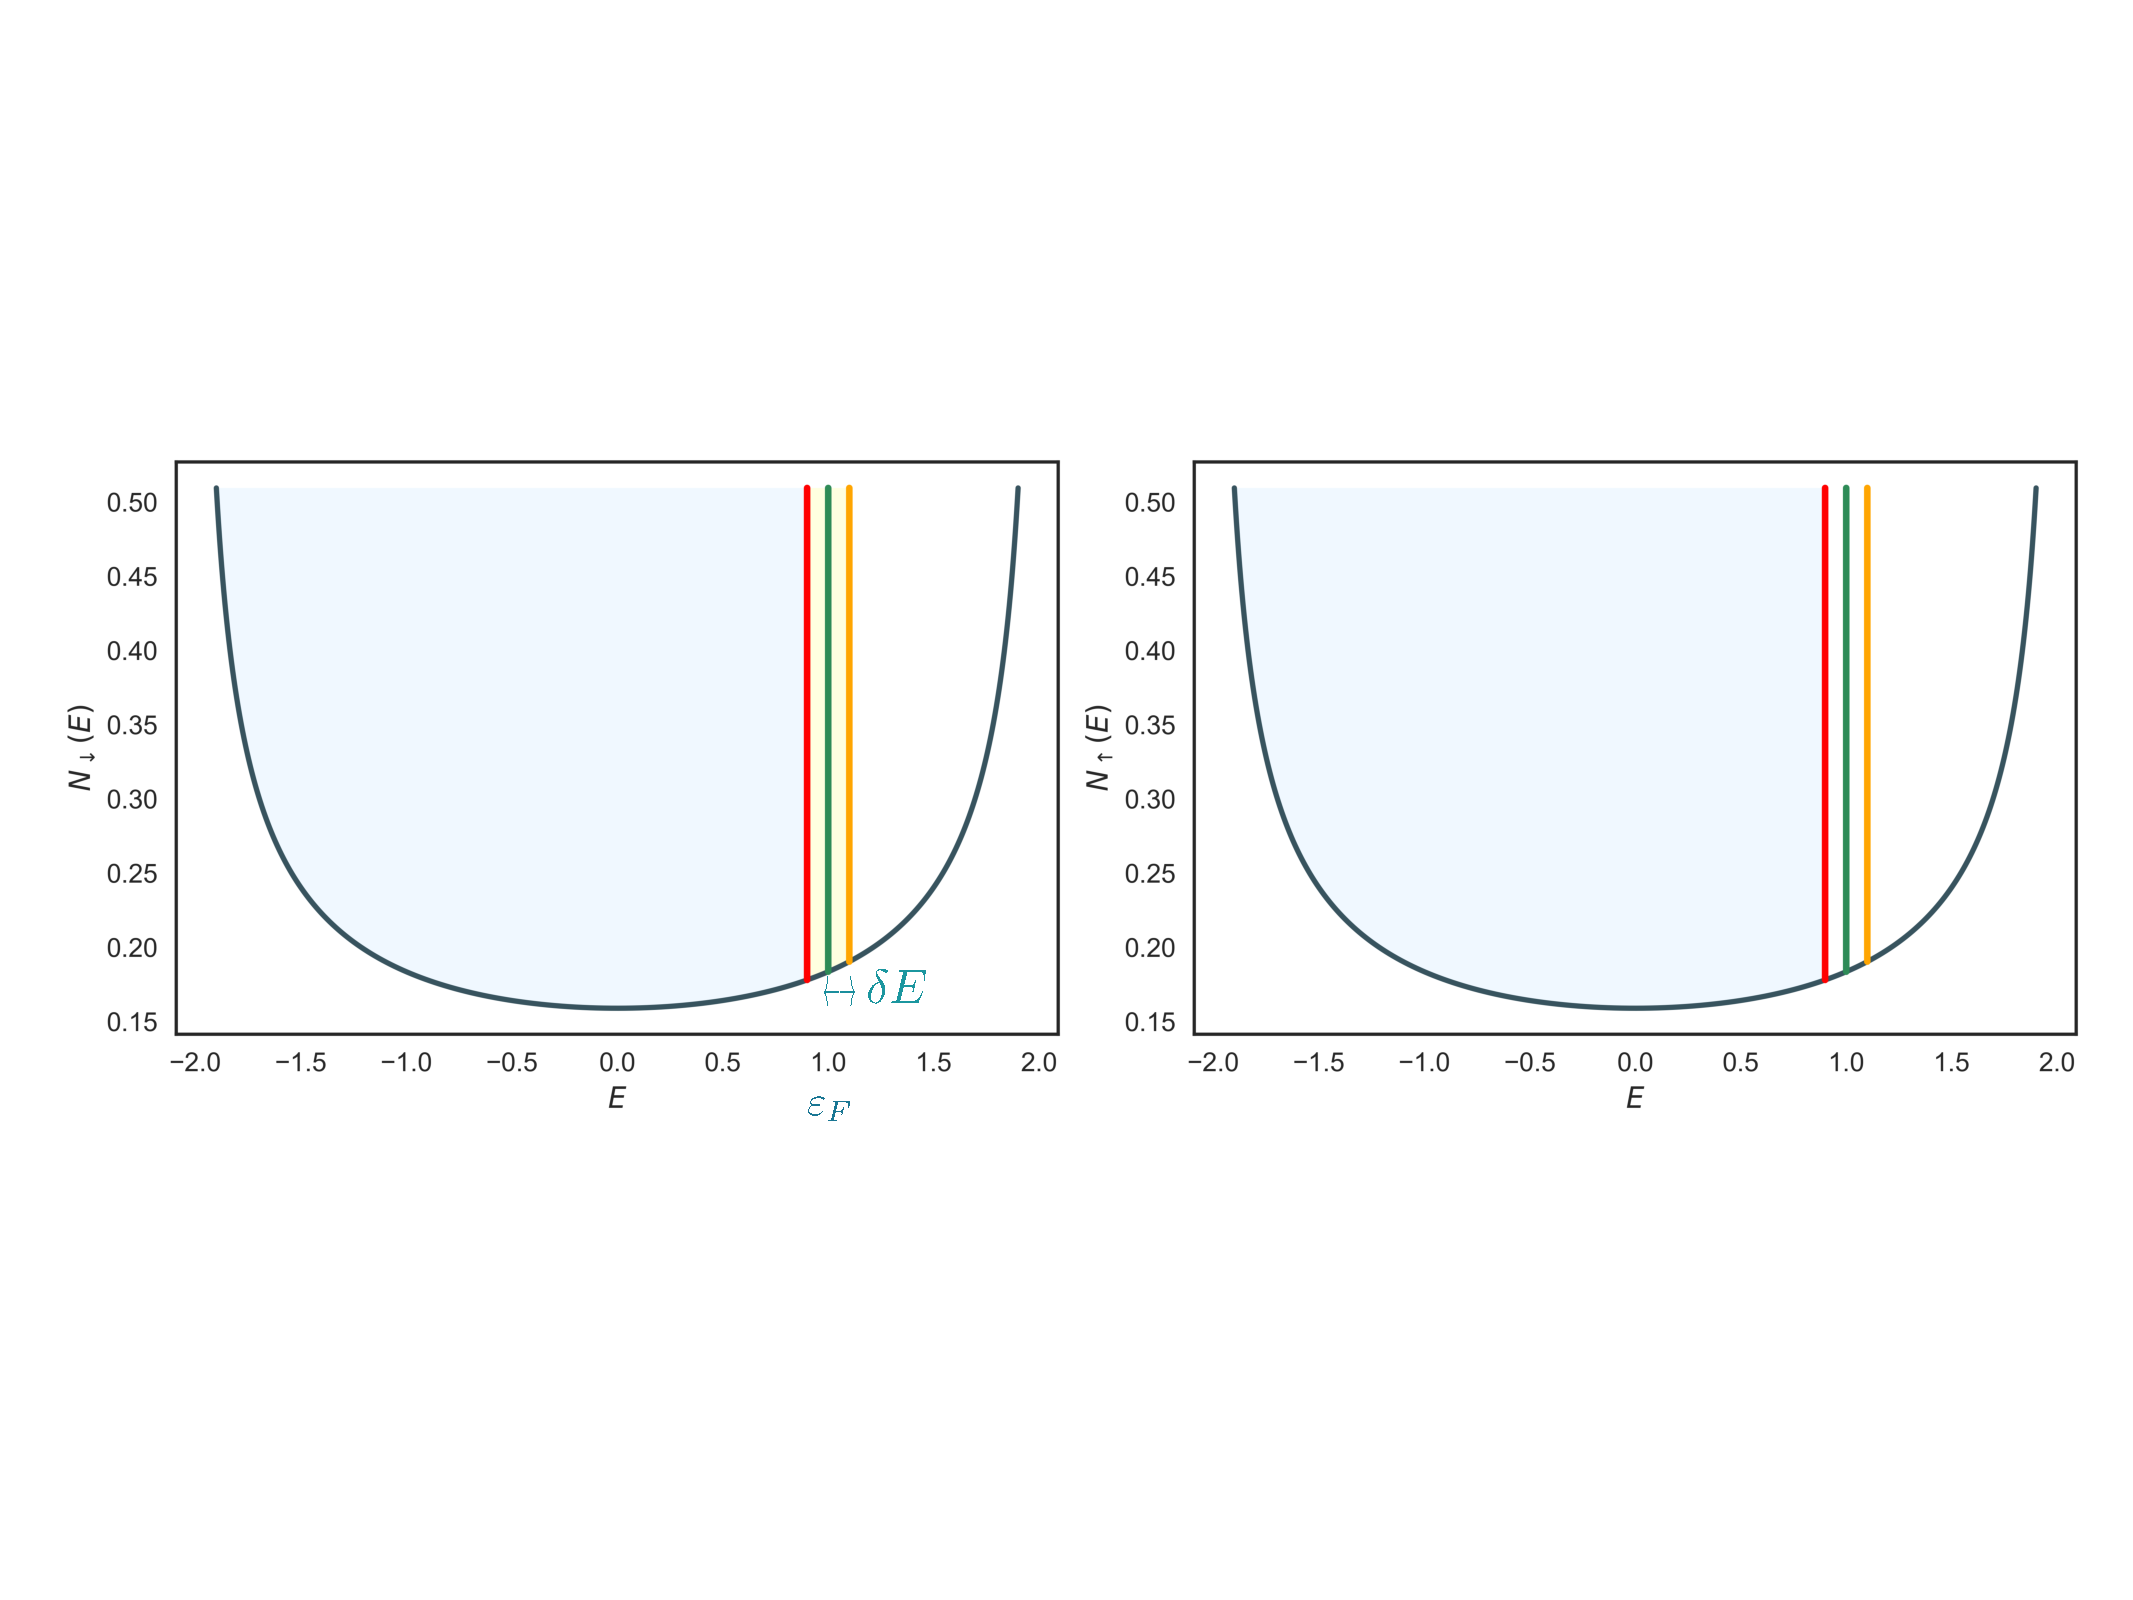
\includegraphics[trim={0 3cm 0 2cm},clip, width=0.7\linewidth]{Hubbard/DOS.pdf}
	\caption[Density of states of the \acs{1D} tight-binding model.]{Density of states of the \acs{1D} tight-binding model.
	Here we represent a polarization of the spins, which leads to an increase in kinetic energy, since the imbalance of spins forces higher energy levels to be filled.}
	\label{fig:dos}
\end{figure}

A system with density of states $N(E)$ has the density of spin-up and spin-down electrons, n, filling the energy levels up to the Fermi energy, $\varepsilon_F$.
When we reduce, say the spin-up electron density by $\delta n$, the potential energy is lowered by $\delta P = U ( n + \delta n ) ( n - \delta n ) - U n^2 = - U (\delta n)^2$.

The extra density of electrons $\delta n$ that is added to the down sector will occupy levels with energy greater than $\varepsilon_F$, so that $\delta n = N ( \varepsilon_F ) \delta E$.
Some spin-up levels below $\varepsilon_F$ that used to be occupied are now empty, which makes $\delta n$ fermions per site increase their energy by $\delta E$, leading to a change in kinetic energy $\delta K = \delta n \delta E = \frac{(\delta n)^2}{N(\varepsilon_F)}$.
The global change in energy is

\begin{equation}
\delta E = \delta P + \delta K = \bigg( - U + \frac{1}{N(\varepsilon_F)} \bigg) \big( \delta n \big)^2 = ( - U N ( \varepsilon_F ) + 1) \frac{(\delta n)^2}{N(\varepsilon_F)}
\end{equation}

If $U N ( \varepsilon_F ) > 1$, then $\delta E < 0$, and the imbalance of spin densities actually becomes more favorable.
Thus, magnetism is favored by a large on-site interaction and a large density of states at (near) the Fermi energy.

\subsection{Mean field theory of the Hubbard model}

We have already encountered an example of a mean field theory when deriving the Hubbard Hamiltonian (see appendix \ref{ap:hartree-fock}, where we provide motivation both heuristically and via a more rigorous variational approach).
In mean field theory, we give a systematic procedure to derive the most plausible quadratic Hamiltonian (which, as we know by now, is soluble) capturing some of the physics of our sytem.
In the case of the Hubbard model, to find the best possible approximation for the quartic term we start by expressing the number operators in terms of an average plus fluctuations: $n = \left\langle n \right\rangle + ( n - \left\langle n \right\rangle ) \equiv \left\langle n \right\rangle + \delta n$.
Then, we make this substitution in the interaction term and neglect the term that is second order in the fluctuations to obtain

\begin{equation}\label{eq:meanFieldNop}
\begin{split}
n_\uparrow n_\downarrow &= \bigg[ \left\langle n_\uparrow \right\rangle + ( n_\uparrow - \left\langle n_\uparrow \right\rangle ) \bigg] \bigg[ \left\langle n_\downarrow \right\rangle + ( n_\downarrow - \left\langle n_\downarrow \right\rangle ) \bigg] \\
&= \left\langle n_\uparrow \right\rangle \left\langle n_\downarrow \right\rangle + \left\langle n_\downarrow \right\rangle ( n_\uparrow - \left\langle n_\uparrow \right\rangle ) + \left\langle n_\uparrow \right\rangle ( n_\downarrow - \left\langle n_\downarrow \right\rangle ) + \mathcal{O}((\delta n)^2) \\
&= n_\uparrow \left\langle n_\downarrow \right\rangle + n_\downarrow \left\langle n_\uparrow \right\rangle - \left\langle n_\uparrow \right\rangle \left\langle n_\downarrow \right\rangle
\end{split}
\end{equation}

We consider a \say{mean field} in the sense that the average density of spin-up electrons interacts with the spin-down electrons and vice-versa.
The last term subtracts the overcounted original single interaction term.
From equation (\ref{eq:meanFieldNop}), we obtain the mean field Hamiltonian

\begin{equation}
\mathcal{H}_{\text{MF}} = - t \sum_{\left\langle i, j \right\rangle, \sigma} \bigg( c_{i\sigma}^\dagger c_{j\sigma} + c_{j\sigma}^\dagger c_{i\sigma} \bigg) + U \sum_i \bigg( n_{i,\uparrow} \left\langle n_{i, \downarrow} \right\rangle + n_{i, \downarrow} \left\langle n_{i, \uparrow} \right\rangle - \left\langle n_{i, \uparrow} \right\rangle \left\langle n_{i, \downarrow} \right\rangle \bigg)
\end{equation}

To solve $\mathcal{H}_{\text{MF}}$, one merely has to diagonalize the corresponding matrix.
In the ferromagnetic case, the average occupation is independent of the specific site, but can vary with the spin species: $n_{i, \uparrow(\downarrow)} = n \Pm m$, where $m$ is the magnetization, the order parameter of the transition to a ferromagnetic phase.

Now we take on a \acl{LG} theory kind of approach.
We compute the energy $E$ for fixed $n$ as a function of $m$, and inspect the system for ferromagnetic ordering: if the minimum lies at $m = 0$, the system is paramagnetic, otherwise it is ferromagnetic.
For simplicity, let us now consider the \acs{1D} model.
Since the average densities are site-independent, we can easily write down the polarized dispersion relations (up to an additive constant):

\begin{equation}\label{eq:meanFieldDispersion}
\varepsilon_{\uparrow k} = U ( n - m ) - 2 t \cos k \quad \varepsilon_{\downarrow k} = U ( n + m ) - 2 t \cos k ,
\end{equation}
and add these levels up for the various possible fillings of the lattice.

The computational procedure to perfom mean field computations goes as follows:
\begin{itemize}
\item Fix the lattice size $N$, the total particle number $N_p$, and the on-site interaction $U$.
\item Set the possible densities by iterating $N_\uparrow = 0, 1, ..., N_p / 2$, and $N_\downarrow = N_p - N_\downarrow$ (we only need half the values since the values are symmetric under $ N_\uparrow \leftrightarrow N_\downarrow$), and setting $n_{\uparrow, \downarrow} = N_{\uparrow, \downarrow} / N$.
\item Fill the lowest $N_\uparrow$, and $N_\downarrow$ energy levels, by looping over the allowes momentum states $k = \frac{2\pi}{N} \{ -\frac{N}{2} + 1, -\frac{N}{2}, ..., \frac{N}{2} \}$, and using equation (\ref{eq:meanFieldDispersion}).
Normalize the energy to $N$ and add in the additive constant $- \left\langle n_\uparrow \right\rangle \left\langle n_\downarrow \right\rangle$.
Out of the energies computed in this way for varying $N_{\uparrow, \downarrow}$, the lowest gives the magnetization for the chosen values of $N_p$ and $U$.
\end{itemize}

\begin{figure}[H]
	\centering
\hspace{12mm}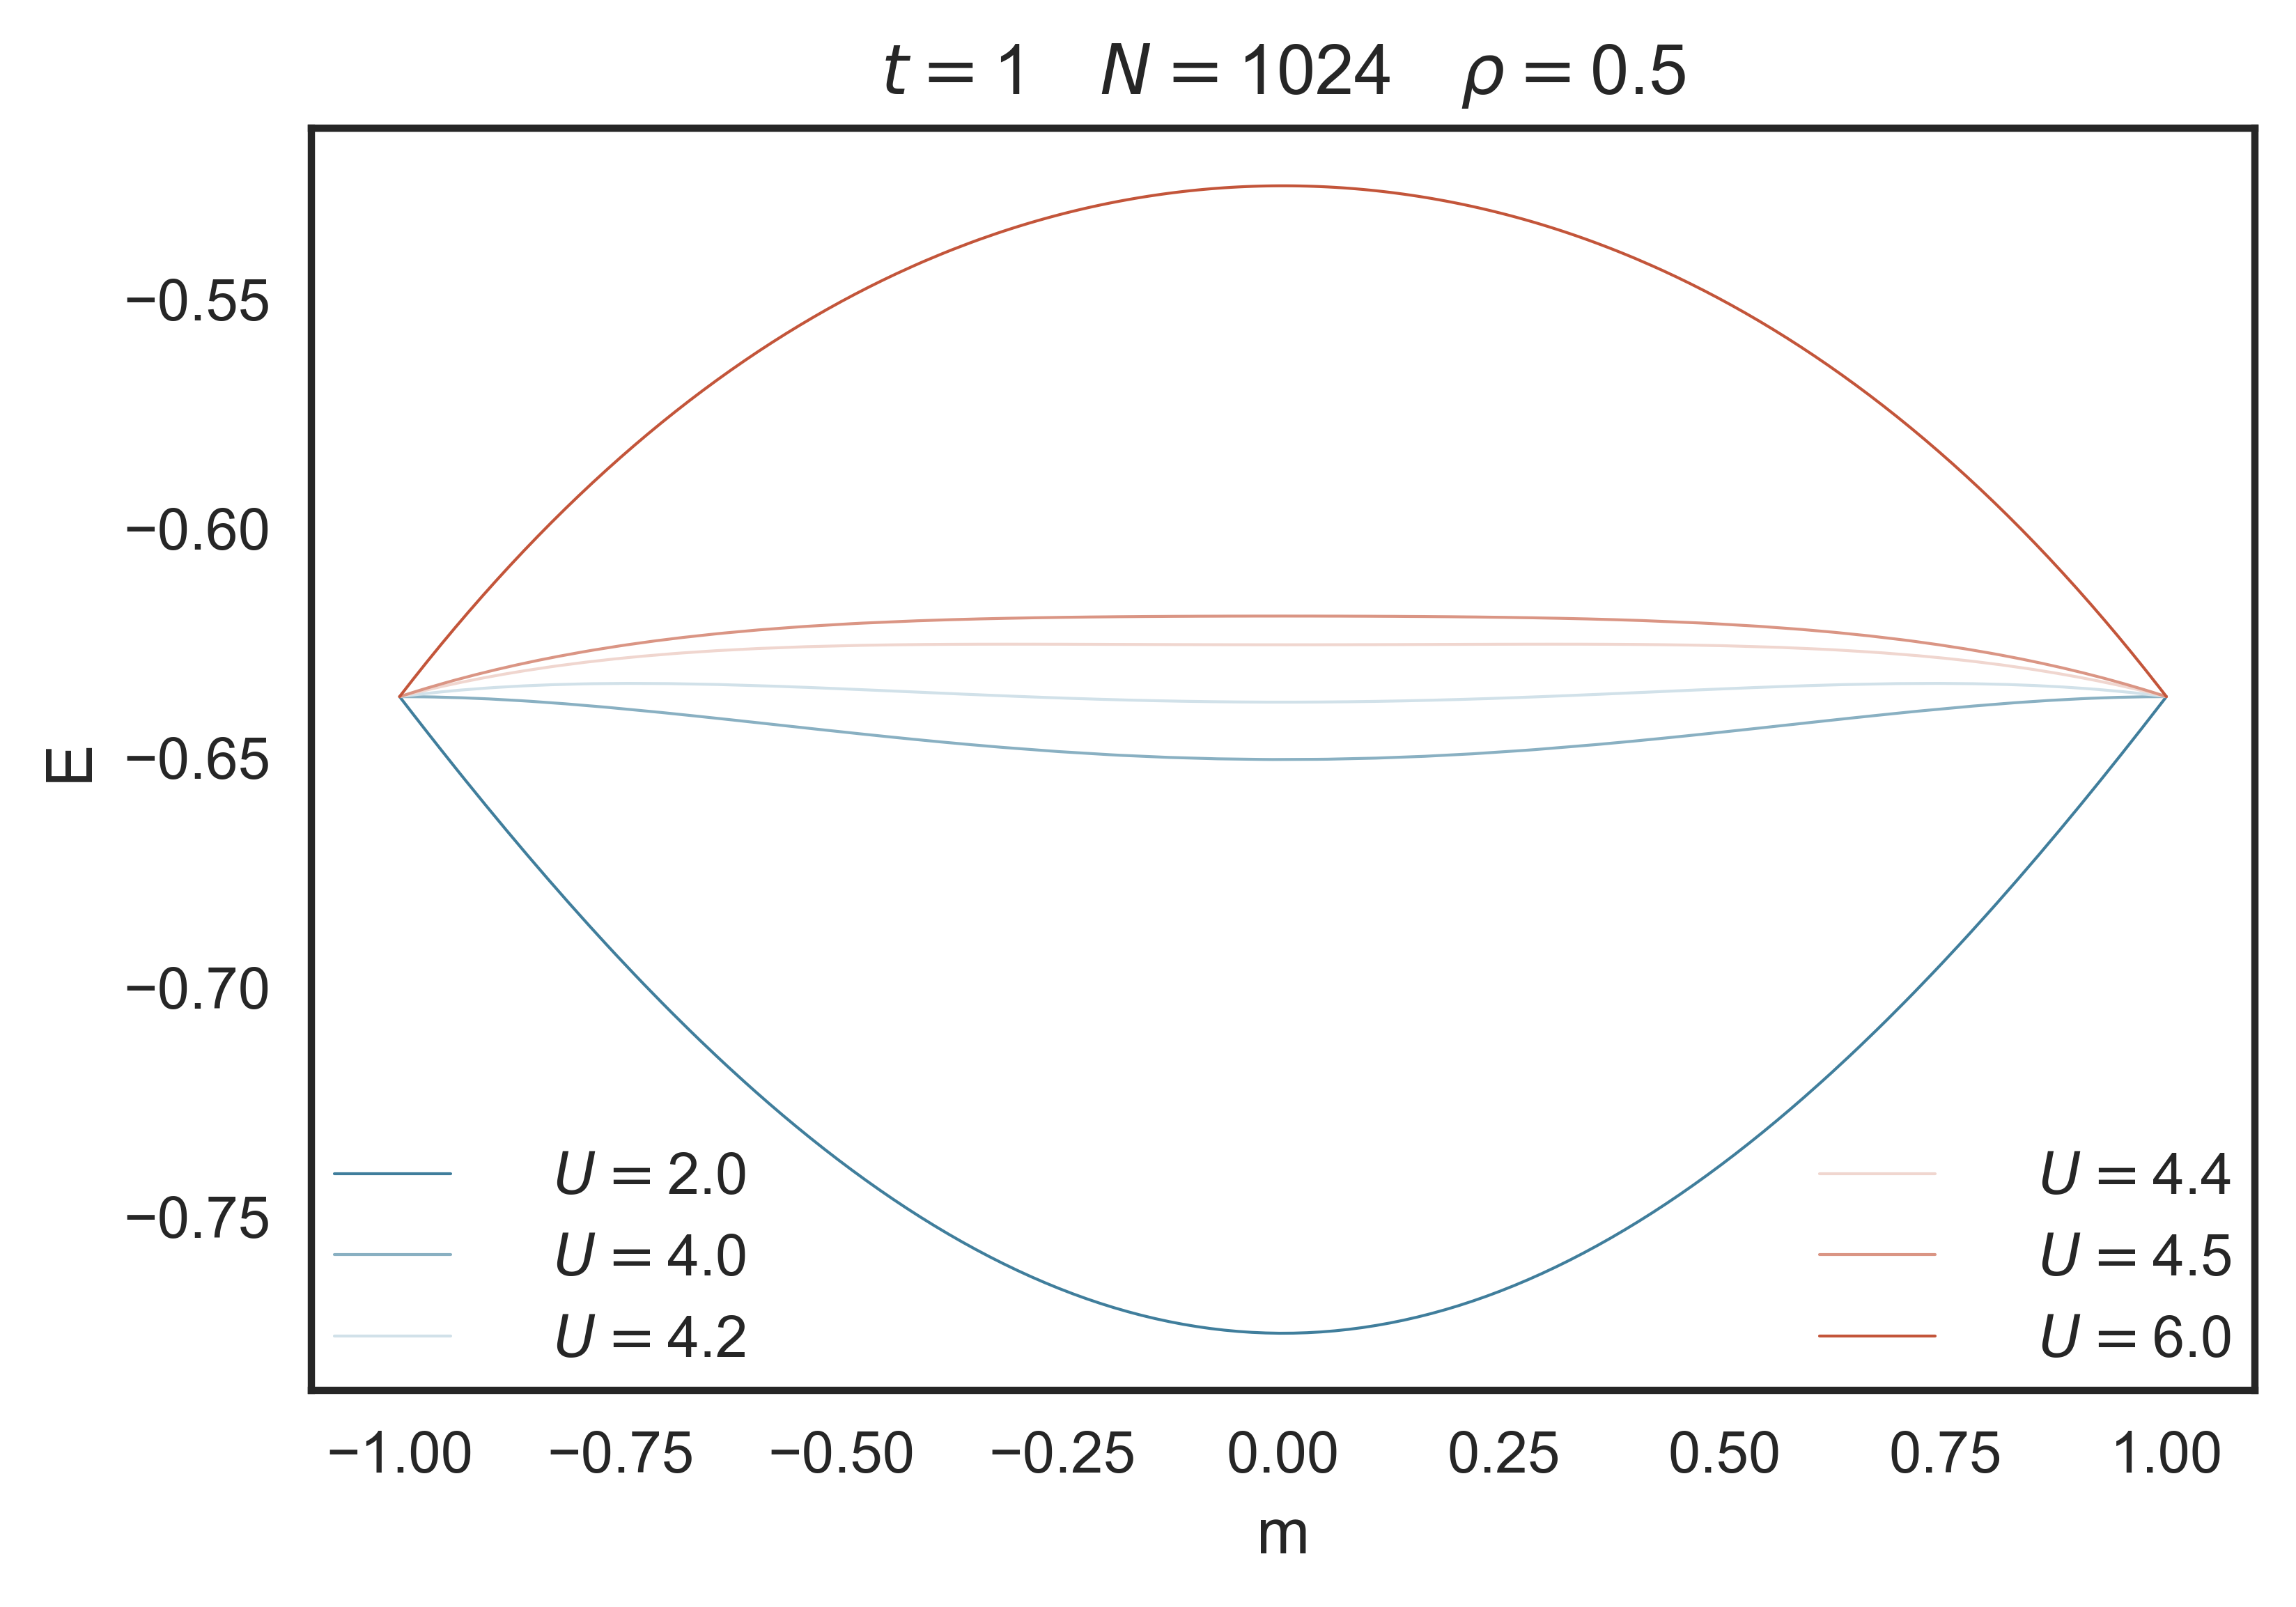
\includegraphics[trim={0 0 0 0},clip, width=0.7\linewidth]{Hubbard/mfHubbard.png}
	\caption[Mean field results for the \acs{1D} Hubbard model.]{Mean field results at quarter filling for a $ 1024$ sites chain.
	$U$ is in units of $t$.
	As the on-site interaction is increased, we see a transition from a paramagnetic to a ferromagnetic phase.}
	\label{fig:mft}
\end{figure}

\begin{figure}[H]
	\centering
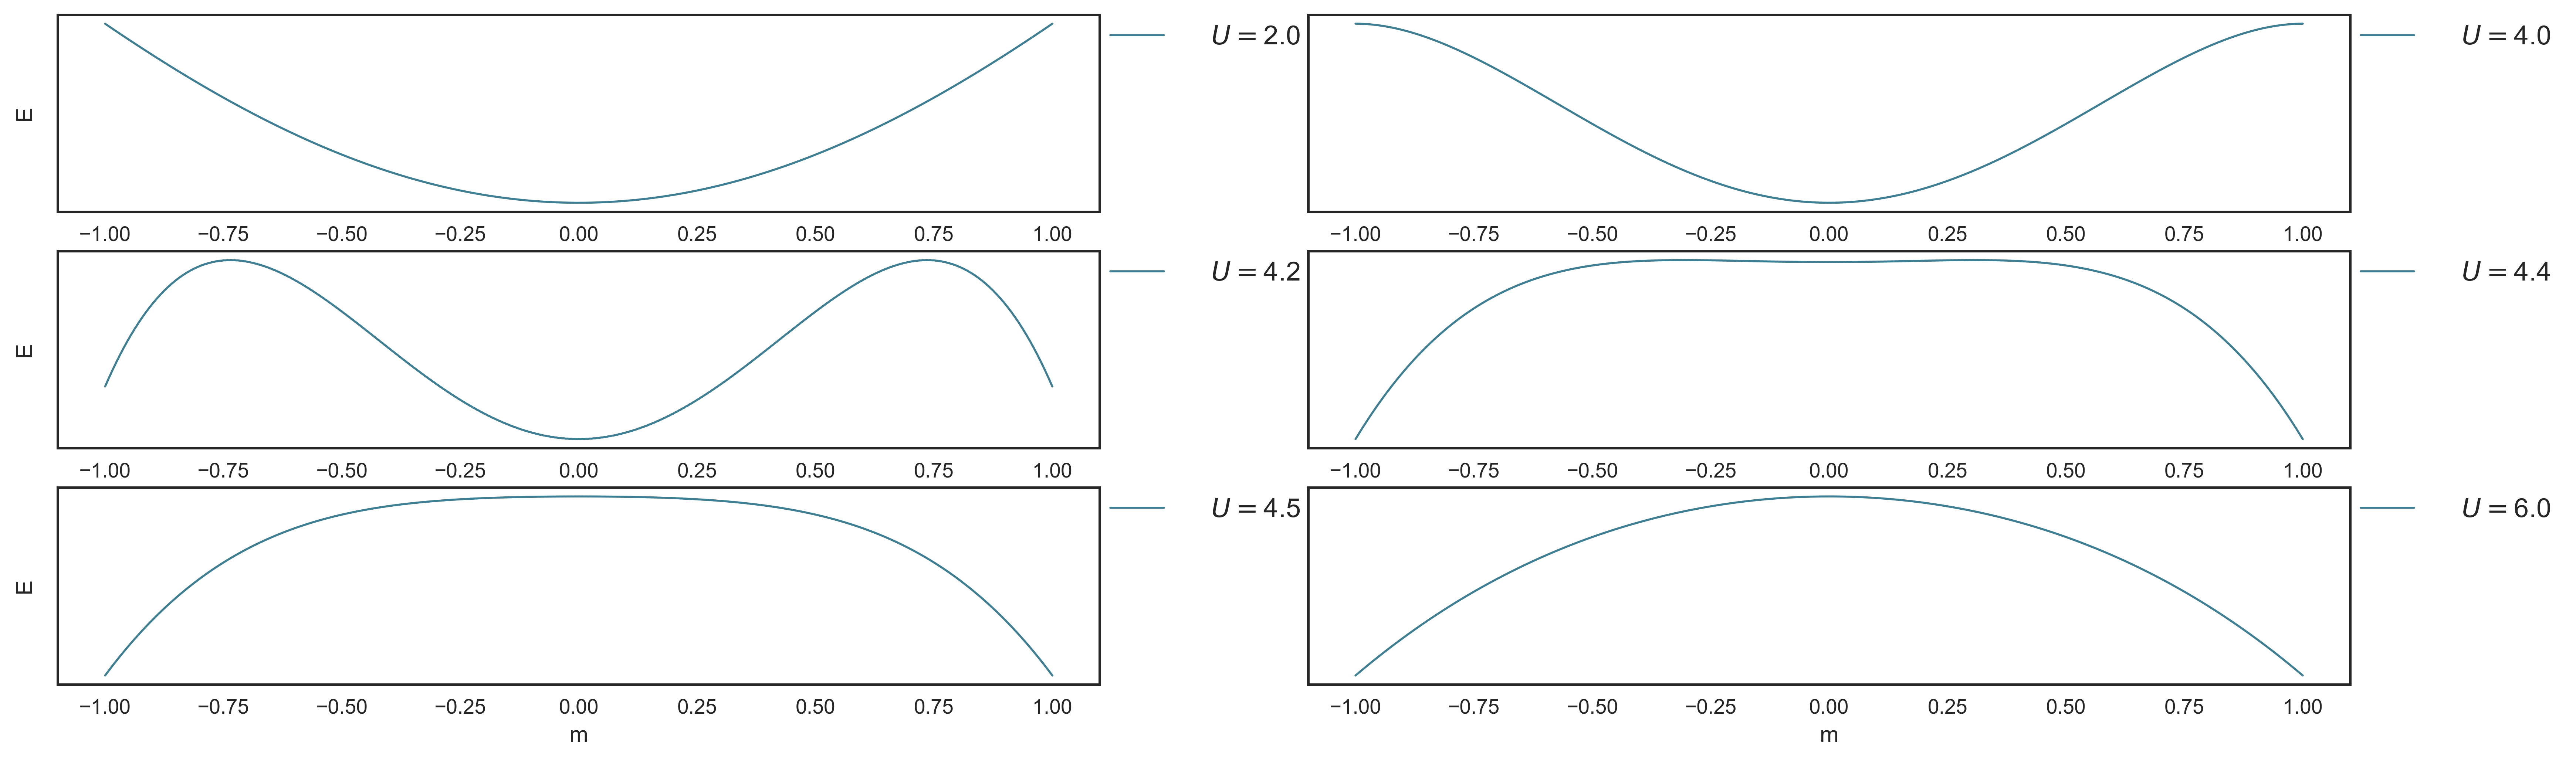
\includegraphics[trim={0 0 0 0},clip, scale = 0.38]{Hubbard/mfHubbard_multiple.png}
	\caption[Mean field results for the \acs{1D} Hubbard model: closing in on the phase transition.]{Mean field}
	\label{fig:mft}
\end{figure}